\section{Паксос}

Алгоритм Паксос (Paxos) считается одним из самых известных методов достижения
консенсуса. Его предложил Лесли Лэмпорт в своей работе The Part-Time
Parliament («Парламент с неполной занятостью») \cite{lamport98}. В данной
статье идея консенсуса была представлена через метафору законодательного
процесса и голосования, происходящих на острове Паксос. Позднее, в 2001 году,
Лэмпорт опубликовал статью Paxos Made Simple («Простой Паксос») \cite{lamport01},
где использовал упрощенную терминологию, которая и используется в данной работе.

В рамках алгоритма Паксос участники могут выполнять одну из трех ролей:

\begin{itemize}
    \item Заявители (proposers). Принимают значения от клиентов, формируют
        предложения для их утверждения и пытаются получить голоса акцепторов.
    \item Акцепторы (acceptors). Участвуют в голосовании за принятие или
        отклонение предложений, сформированных заявителями. Для устойчивости
        к отказам система включает несколько акцепторов, однако для принятия
        решения достаточно кворума (то есть большинства голосов).
    \item Ученики (learners). Отвечают за хранение результатов принятых решений,
        выполняя роль реплик.
\end{itemize}

В большинстве реализаций эти роли совмещены в одном процессе.

Каждое предложение содержит уникальный номер, который монотонно увеличивается,
и значение, предложенное клиентом. Номер предложения используется для установления
общего порядка операций и определения их последовательности («до» или «после»).
Номера предложений часто оформляются как пара (идентификатор узла и временная метка).
Идентификаторы узлов являются упорядочиваемыми и могут быть использованы для
разрешения конфликтов между временными метками. Для корректной работы алгоритма
требуется синхронизация локальных часов.

\subsection{Алгоритм Paxos}

Алгоритм Паксос можно разделить на два ключевых этапа: голосование (или этап
предложения) и репликацию. На этапе голосования заявители борются за установление
своего лидерства, а на этапе репликации заявитель распространяет согласованное
значение среди акцепторов.

Заявитель выступает как начальная точка контакта для клиента, получая значение,
которое должно быть принято, и пытается собрать голоса от акцепторов. После
этого акцепторы рассылают информацию о принятом значении среди учеников, что
позволяет ответить пользователю. Ученики, в свою очередь, увеличивают
коэффициент репликации согласованного значения.

Только один заявитель может получить большинство голосов. В случае, если
голоса распределяются равномерно, ни один из заявителей не сможет набрать
большинство, и тогда им придется начать процесс заново.

На этапе предложения заявитель отправляет запрос $Подготовка(n)$ (где $n$ —
номер предложения) большинству акцепторов, пытаясь собрать их голоса. Акцептор,
получив запрос, должен ответить, соблюдая несколько инвариантов \cite{lamport01}:

\begin{itemize}
    \item Если акцептор еще не отвечал на запрос с более высоким порядковым
        номером, он обещает не принимать предложения с меньшими номерами.
    \item Если акцептор уже принял какое-то предложение, он уведомляет
        заявителя о принятом значении через сообщение $Обещание(m, v_{\text{принятых}})$.
    \item Если акцептор ранее ответил на запрос с большим порядковым номером, он
        уведомляет заявителя о существующем предложении с более высоким номером.
    \item Акцептор может ответить на несколько запросов, если последний имеет
        наибольший порядковый номер.
\end{itemize}

Когда заявитель получает большинство голосов, начинается этап репликации.
Заявитель фиксирует предложение, отправляя акцепторам сообщение $Принятие(n, v)$,
где $v$ — это значение, соответствующее предложению с наибольшим номером среди
полученных ответов от акцепторов, или собственное значение заявителя, если
акцепторы не приняли других предложений.

Акцептор примет предложение с номером $n$, если на этапе предложения он не
ответил на запрос с большим номером. Если акцептор отклоняет предложение, он
отправляет заявителю максимальный порядковый номер, который он видел, для
актуализации данных заявителя \cite{lamport01}.

Обобщенная схема раунда Паксос приведена на рис \ref{fig:paxos}.

\begin{figure}
  \centering
  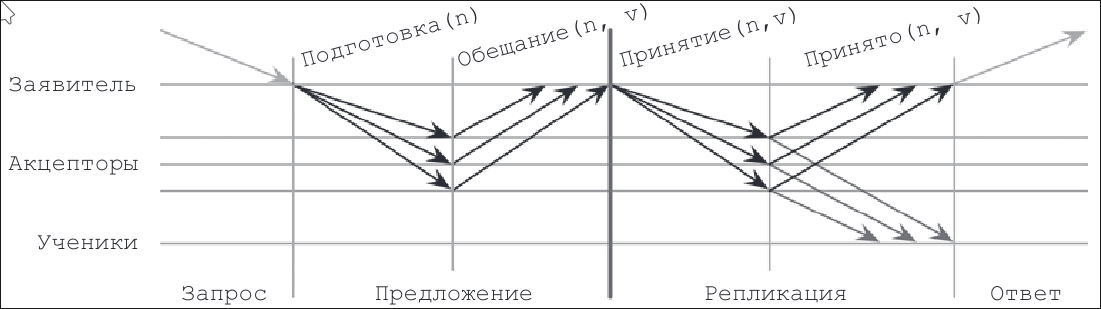
\includegraphics[scale=0.4]{inc/paxos.png}
  \caption{Схема раунда Паксос}
  \label{fig:paxos}
\end{figure}

После того как консенсус относительно значения достигнут (хотя бы один акцептор
принял решение), последующие заявители должны принять это значение, чтобы
сохранить согласованность. Поэтому акцепторы возвращают последнее принятое
значение. Если ни один акцептор не видел предыдущего значения, заявителю
разрешается выбрать собственное.

Ученики получают информацию о принятом значении, когда большинство акцепторов
сообщает им об этом. Акцепторы могут сразу уведомить учеников о принятом
значении. При наличии нескольких учеников акцепторы должны уведомить каждого,
однако можно выделить несколько учеников, которые будут отвечать за
уведомление других.

Таким образом, основной целью первого этапа алгоритма является установление
лидера и определение принятого значения, что позволяет перейти ко второму
этапу — распространению значения. В базовом алгоритме оба этапа выполняются
каждый раз, когда необходимо принять решение. Однако на практике можно
уменьшить количество шагов. Этот подход будет рассмотрен позже в разделе
"Мульти-Паксос".

\subsection{Мульти-Паксос}

Ранее мы рассматривали классический Паксос, в котором любой узел может стать
заявителем и инициировать раунд. Проблема этого подхода в том, что для каждого
нового раунда репликации требуется запускать стадию предложения (этап с
Подготовкой). Чтобы избежать таких повторений и дать заявителю возможность
многократно использовать своё положение, применяется мульти-Паксос \cite{lamport01}.
Он вводит роль лидера — выделенного заявителя, который после утверждения может
сразу приступать к репликации, минуя стадию предложения.

В классическом Паксосе чтение часто реализуется через дополнительный раунд,
собирающий любые незавершённые данные, поскольку нет гарантии, что последний
заявитель имеет самую свежую версию состояния. В мульти-Паксосе появляется
сходная проблема: если мы читаем данные у лидера, который уже успел смениться,
то можем получить устаревшую информацию. Чтобы этого избежать и поддерживать
линеаризуемость, некоторые реализации используют механизм аренды (lease)
\cite{chandra07}. Лидер периодически подтверждает свою активность, а узлы
обещают не принимать другие предложения в течение срока аренды. Этот приём не
гарантирует абсолютную корректность, но ускоряет операции чтения при условии
ограниченной синхронизации часов. Однако в случае рассинхронизации часов, когда
лидер считает, что его срок аренды не истек, а другие участники - наоборот,
линеаризуемость недостижима.

Мульти-Паксос обычно описывают как реплицируемый журнал операций над некоторой
структурой. При сбоях участники восстанавливают данные из долговременного журнала
сообщений. Чтобы журнал не разрастался бесконечно, принято периодически
создавать моментальные снимки состояния (снапшоты) и усекать журнал до отметки
этого снимка.
